% Guava Fruit Disease Classification -- full report (8-10 pages)
% Compile from report/:  ../bin/tectonic report.tex
\documentclass[11pt,a4paper]{article}
\usepackage[T1]{fontenc}
\usepackage{lmodern}
\usepackage[margin=2.2cm]{geometry}
\usepackage{graphicx}
\usepackage{booktabs}
\usepackage{amsmath,amssymb}
\usepackage{natbib}
\usepackage[colorlinks=true,linkcolor=blue,citecolor=blue,urlcolor=blue]{hyperref}
\usepackage{xcolor}
\usepackage{caption}
\usepackage{float}
\usepackage{subcaption}
\usepackage{tikz}
\usetikzlibrary{positioning,arrows.meta}
\usepackage{array}
\usepackage{multirow}
\graphicspath{{../outputs/plots/}{../outputs/audit/}}
\setlength{\parskip}{2pt}
\setlength{\parindent}{0pt}
\captionsetup{font=small,labelfont=bf}

\title{\vspace{-1.2cm}\textbf{Guava Fruit Disease Classification with a Leakage-Aware Evaluation:\\
A Custom CNN versus Two-Phase EfficientNetB0 Transfer Learning}}
\author{Nihar Ranjan Mishra \and Aaviraj Nikumbh \and Neel Lakhani}
\date{October 2026}

\begin{document}
\maketitle

\begin{abstract}
\noindent
We classify guava fruit images from the public GFDD24 dataset into
Anthracnose, Fruit Flies, and Healthy, and compare a compact CNN trained from
scratch (Model A) with two-phase ImageNet transfer learning (Model B), using a
controlled backbone comparison over MobileNetV2, EfficientNetB0, and ResNet50;
EfficientNetB0 is selected by leak-free validation. The released GFDD24 splits
are not independent: each of 473 source
fruits was augmented eight times \emph{before} splitting, so 100\% of
validation and test images share a source original with training. We quantify
this leakage and build a cluster-grouped leak-free re-split as a control. All
model selection is performed on leak-free validation data; the leak-free test
split is touched only for final configurations. We fix an early-stopping bug
that stopped Model A while validation accuracy was still improving, then run a
controlled optimisation study over optimiser, learning rate, fine-tuning depth,
and backbone, followed by three seeds per final configuration. Every number in
this report is produced by an executed run logged in
\texttt{outputs/logs/}. We report bootstrap confidence intervals, Wilson
intervals, and exact McNemar tests on paired per-image predictions, and we
state explicitly when a difference is within one or two test images. Grad-CAM
panels for both models support the quantitative comparison. The result is a
reproducible, leakage-aware baseline for guava disease classification rather
than another single-split leaderboard entry.
\vspace{0.3em}

\noindent\textbf{Keywords:} guava disease classification; GFDD24; transfer
learning; EfficientNetB0; data leakage; Grad-CAM; McNemar test;
reproducibility.
\end{abstract}

\section{Introduction}
Guava (\textit{Psidium guajava}) is an economically important fruit crop in
South Asia, and anthracnose and fruit-fly damage are among the most visible
causes of post-harvest loss. A phone photograph is a cheap sensor; the open
question is whether a learned classifier can be trusted when it is deployed on
fruit from a new orchard. Public benchmarks usually report a single accuracy
on a curated split, which is a necessary but insufficient answer.

This project asks three questions. First, how much does a from-scratch CNN
lose relative to ImageNet-pretrained transfer models on a small three-class
fruit dataset? Second, how much of the reported accuracy is an artefact of
data leakage caused by augmenting before splitting? Third, which optimiser,
learning-rate, and fine-tuning-depth choices survive a controlled comparison
when all tuning is done on a leak-free validation split?

Our contributions are: (i) a quantified leakage audit of GFDD24 and a
cluster-grouped leak-free re-split; (ii) a fixed, early-stopping-corrected
Model A baseline; (iii) a controlled optimisation grid (E1--E5) and three-seed
final runs (E6) for both models; (iv) paired statistical tests with confidence
intervals; and (v) Grad-CAM evidence for correct and misclassified examples.
We deliberately do not claim state-of-the-art accuracy: the dataset is small,
the build is CPU-only, and the leak-free control is the scientific point.

\section{Literature review}
Plant-disease recognition with CNNs is a mature subfield. \citet{mohanty2016plant}
showed that AlexNet and GoogLeNet can exceed 99\% on the curated PlantVillage
benchmark, while accuracy drops on field photographs from other sources. That
gap between curated and field performance is the motivation for our leak-free
control. GFDD24 \citep{gfdd24} is a recent three-class guava fruit dataset with
field photographs and a released train/validation/test split; its augmentation
was applied before splitting, which is the data-centric problem we audit.

Architecturally, MobileNetV2 \citep{sandler2018mobilenetv2} is a strong
accuracy-per-FLOP choice for mobile vision: inverted residual blocks with
linear bottlenecks. EfficientNetB0 \citep{tan2019efficientnet} uses compound
scaling of depth, width, and resolution, while ResNet50
\citep{he2016resnet} provides a deeper residual baseline. We compare all three
under the same two-phase protocol. Transfer learning from ImageNet
\citep{russakovsky2015imagenet} is justified by the feature-transfer results of
\citet{yosinski2014transfer}: early filters are general, later layers
specialise, and fine-tuning adapts them to a target domain. Our Model A follows
the standard small-data recipe with batch normalisation
\citep{ioffe2015bn} and dropout \citep{srivastava2014dropout}; our Model B uses
the same two-phase protocol (frozen head warm-up, then fine-tuning) that is
standard for small agricultural datasets.

Several guava studies report high curated-split accuracy: Mostafa et al.\
\citep{mostafa2021guava} compare five CNNs on a five-class guava set,
Doutoum et al.\ \citep{doutoum2023guava} compare transfer backbones on guava
leaves, Nandi et al.\ \citep{nandi2022device} target edge deployment with
quantisation, Kilci and Koklu \citep{kilci2024squeezenet} combine SqueezeNet
features with boosting on GFDD24, and Zhou \citep{zhou2026guava} reports a
six-way transfer comparison with Grad-CAM. A ResNet-101 + Grad-CAM study
\citep{resnet101guava2025} and a CNN--boosting ensemble
\citep{cnnGBensemble2025} also report GFDD24 numbers, and Pratama et al.\
\citep{pratama2025jessi} compare MobileNetV2 transfer for guava disease
detection. These papers establish that transfer learning works; they do not,
as a group, report a from-scratch versus two-phase transfer head-to-head with
a cross-split duplicate audit, a leak-free control, and paired statistics on
the same test images. That narrower gap is what this report fills.

Leakage is not a hypothetical concern. \citet{tampu2022leakage} showed that
splitting two-dimensional slices from the same OCT volume across train and
test inflated accuracy by 5--30 percentage points. GFDD24's eight augmented
views per fruit are structurally analogous: eight views of one fruit are eight
slices of one volume. Our audit confirms that the released split places those
views on both sides of the train/test boundary.

\section{Methodology}
\subsection{Dataset and leakage audit}
GFDD24 contains 3,784 $512\times512$ RGB PNG images from three classes
(Anthracnose, Fruit Flies, Healthy), derived from 473 source fruits with eight
augmented variants each. The released split has 2,647 training, 755 validation,
and 382 test images on disk (the release notes state 775 validation images; we
report the 20-image discrepancy rather than hiding it). All images were
verified readable and correctly sized in the audit.

The leakage audit keys each file by its source-original identifier, using the
full timestamp for the timestamp-named fruit-fly files and the leading integer
for the other files. It finds 454 of 473 originals (96\%) with variants in more
than one split, and 100\% of validation and test images share an original with
the training set. The released test score is therefore a near-duplicate
recognition score, not a field-generalisation score.

To measure the gap, we build \texttt{Dataset\_leakfree/}: originals are grouped
into clusters and assigned 70/20/10 to train/validation/test, so no cluster
spans splits (0 of 473). The leak-free split contains 2,632 training, 760
validation, and 392 test images, versus 2,647/755/382 for the released split.
All tuning below uses the leak-free training split to fit and the leak-free
validation split to select. The leak-free test split is evaluated once for the
final configurations and once for the fixed Model A required by Task~1.

\subsection{Model A: custom CNN}
Model A is a four-block convolutional network. Each block applies two
$3\times3$ convolutions with ReLU and batch normalisation, followed by
$2\times2$ max-pooling and dropout 0.25; the filter counts are 32, 64, 128, and
256. Global average pooling is followed by a 256-unit dense layer, batch
normalisation, dropout 0.5, and a three-way softmax. The model has 1.24M
parameters. Batch-normalisation momentum is 0.9 rather than the Keras default
0.99; with Adam at $10^{-3}$ the network learns quickly enough that
momentum-0.99 moving averages lag the batch statistics, and inference collapsed
to a single class in an earlier run. The fix is documented as a bug lesson,
not hidden as a tuning choice.

\subsection{Model B: two-phase ImageNet transfer}
Model B uses an ImageNet-pretrained backbone without its top layer. The input
is passed through the frozen backbone, global average pooled, projected to 256
units, dropped out at 0.4, and classified by a three-way softmax. Phase~1
trains the head with the backbone frozen. Phase~2 unfreezes the last 30
backbone layers (batch-normalisation layers stay frozen) and fine-tunes at a
lower learning rate. MobileNetV2 is the reference backbone; E4 also trains
EfficientNetB0 and ResNet50 under the same protocol. EfficientNetB0 is selected
by leak-free validation and is the final Model B. Its best checkpoint is from
phase~1, so the final model is a frozen EfficientNetB0 feature extractor plus
the 256-unit head (4.38M parameters, 0.33M trainable); fine-tuning did not
improve it. MobileNetV2 has 2.59M parameters (1.84M trainable in phase~2), and
ResNet50 has 24.1M. Preprocessing is backbone-specific: MobileNetV2 uses
$[-1,1]$, EfficientNetB0 uses $[0,255]$ because its own layers rescale, and
ResNet50 uses an RGB-order mean-subtraction approximation (no BGR flip).

\begin{figure}[t]
\centering
\resizebox{\textwidth}{!}{%
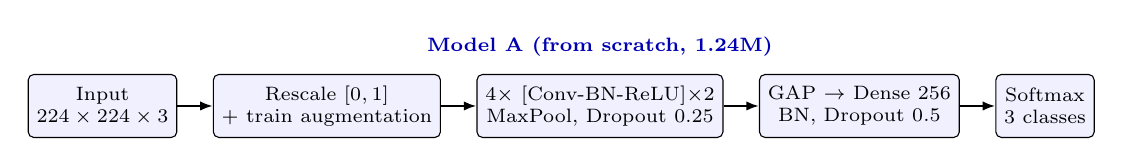
\begin{tikzpicture}[font=\scriptsize, node distance=4.5mm,
  box/.style={draw, rounded corners=2pt, align=center, minimum height=8mm,
              fill=blue!6, inner sep=3pt},
  arr/.style={-{Latex[length=1.6mm]}, thick}]
\node[box] (in) {Input\\$224\times224\times3$};
\node[box, right=of in] (aug) {Rescale $[0,1]$\\+ train augmentation};
\node[box, right=of aug] (a) {4$\times$ [Conv-BN-ReLU]$\times2$\\MaxPool, Dropout 0.25};
\node[box, right=of a] (gap) {GAP $\to$ Dense 256\\BN, Dropout 0.5};
\node[box, right=of gap] (out) {Softmax\\3 classes};
\draw[arr] (in) -- (aug); \draw[arr] (aug) -- (a);
\draw[arr] (a) -- (gap); \draw[arr] (gap) -- (out);
\node[above=1mm of a, text=blue!70!black] {\textbf{Model A (from scratch, 1.24M)}};
\end{tikzpicture}}

\vspace{2mm}
\resizebox{\textwidth}{!}{%
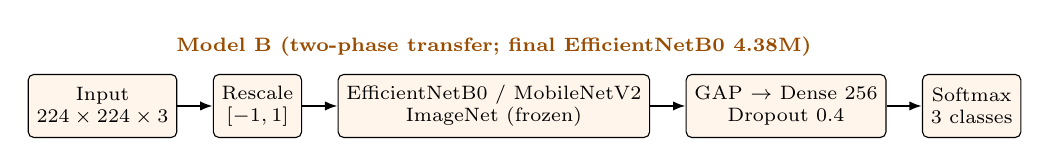
\begin{tikzpicture}[font=\scriptsize, node distance=4.5mm,
  box/.style={draw, rounded corners=2pt, align=center, minimum height=8mm,
              fill=orange!8, inner sep=3pt},
  arr/.style={-{Latex[length=1.6mm]}, thick}]
\node[box] (in2) {Input\\$224\times224\times3$};
\node[box, right=of in2] (pre) {Rescale\\$[-1,1]$};
\node[box, right=of pre] (bb) {EfficientNetB0 / MobileNetV2\\ImageNet (frozen)};
\node[box, right=of bb] (gap2) {GAP $\to$ Dense 256\\Dropout 0.4};
\node[box, right=of gap2] (out2) {Softmax\\3 classes};
\draw[arr] (in2) -- (pre); \draw[arr] (pre) -- (bb);
\draw[arr] (bb) -- (gap2); \draw[arr] (gap2) -- (out2);
\node[above=1mm of bb, text=orange!60!black] {\textbf{Model B (two-phase transfer; final EfficientNetB0 4.38M)}};
\end{tikzpicture}}
\caption{Block diagrams. Model A is trained from scratch. Model B first trains
the head with the backbone frozen (phase~1), then unfreezes the last 30
backbone layers at a lower learning rate (phase~2); batch-normalisation layers
remain frozen in both phases. The final EfficientNetB0 checkpoint is the
phase~1 model, so the deployed classifier is a frozen feature extractor plus
the head.}
\label{fig:architecture}
\end{figure}

\subsection{Training protocol and optimisation grid}
All runs use seed 42 unless stated, $224\times224$ inputs, batch size 32, and
categorical cross-entropy. The training split is augmented in-graph with
horizontal/vertical flips, rotation ($\pm15\%$), zoom ($\pm15\%$), contrast, and
brightness; validation and test are only rescaled to $[0,1]$. The brightness
and contrast layers use \texttt{value\_range=(0,1)} because they otherwise
default to $[0,255]$ and skew training inputs away from validation inputs (a
bug we found and fixed; see Section~\ref{sec:bugs}).

Model selection uses validation accuracy, not validation loss. Early stopping
has patience 8 and restores the best weights; the fixed Model A run is forced
to run at least 15 epochs. E1 uses the task-specified 8 head epochs plus 8
fine-tuning epochs. E2--E4 use 6+6 epochs because the two-stream CPU budget
was the binding constraint; this is an explicit cut (DECISIONS D12), not a
silent grid shrinkage. The final configurations use the selected schedule with
three seeds (42, 43, 44). Every run writes a JSON metadata file
with the full configuration, per-run CSV history, best checkpoint, and
save/reload parity check; rerunning a completed tag is skipped.

The optimisation study is:
\begin{itemize}
  \item \textbf{E1 (optimiser, Model B):} Adam, AdamW, SGD with Nesterov
        momentum 0.9, RMSprop at the reference learning rates (SGD uses
        $10^{-2}$ head / $10^{-3}$ fine-tune as specified).
  \item \textbf{E2 (learning rate, one factor at a time):} head
        $\{10^{-2},10^{-3},3\times10^{-4}\}$ and fine-tune
        $\{10^{-4},10^{-5},10^{-6}\}$, with the reference value for the other
        phase.
  \item \textbf{E3 (fine-tune depth):} unfreeze last $\{0,30,60,\text{all}\}$
        backbone layers.
  \item \textbf{E4 (backbone):} MobileNetV2, EfficientNetB0, ResNet50 with the
        same two-phase protocol; we log parameters, minutes per epoch, and
        single-image inference latency.
  \item \textbf{E5 (Model A):} Adam, SGD, and a cosine-decay schedule at an
        8-epoch budget (task cap 12). AdamW and RMSprop for Model A were cut
        because each additional run costs roughly 30--50 CPU minutes; the cut
        is recorded in \texttt{DECISIONS.md} D13.
  \item \textbf{E6 (final configurations):} EfficientNetB0 for Model B and the
        fixed-A protocol for Model A, trained with seeds 42, 43, and 44. The
        8-epoch E5 winner was tested and rejected as undertrained (D19). Test
        accuracy is reported as mean $\pm$ standard deviation, with bootstrap
        confidence intervals for each run.
\end{itemize}

\subsection{Statistical analysis}
For every final run we save per-image predictions on the identical test
images. We report percentile bootstrap 95\% confidence intervals (2,000
resamples, seed 42) for accuracy and macro-F1, Wilson score intervals for
accuracy, and exact two-sided McNemar tests on paired correctness. A difference
is described as ``within noise'' when the McNemar test is not significant at
$\alpha=0.05$, and separately when the absolute difference is at most one or
two test images even if the test is significant. This prevents over-reading
small differences on a 392-image test set.

\section{Results and discussion}
\subsection{Fixing Model A}
The original Model A run used early stopping on validation loss. Validation
loss was lowest at epoch~1, so training stopped at epoch~9 even though
validation accuracy was still improving; the reported test accuracy was 0.9110.
We reran Model A with early stopping on validation accuracy, patience 8, a
minimum of 15 epochs, and best-weight restoration. The fixed run scores 0.9634
on the released split and 0.9923 on the leak-free split; both rows are in
Table~\ref{tab:final}. This is the correct baseline for the A-versus-B
comparison. The original run is kept only as provenance: its metrics JSON
survives, but its checkpoint and CSV log were later overwritten by a smoke test
that reused the default tag (D14), so it is not used for paired tests.

\subsection{Optimisation experiments}
Table~\ref{tab:grid} summarises the validation-only grid. No test split was
touched during E1--E5; the best configuration in each family is selected by
leak-free validation accuracy, with training cost as a secondary criterion.

\begin{table}[H]\centering\small
\caption{Validation-only optimisation grid. E1 uses 8+8 epochs; E2--E4 use the
same 6+6 budget and the E2 reference (MobileNetV2, Adam, matched learning
rates); E5 uses an 8-epoch budget. Best epoch is the epoch of best validation
accuracy.}
\label{tab:grid}\begin{tabular}{lccc}
\toprule
Setting & Best val acc & Best epoch & Min \\
\midrule
\addlinespace
\multicolumn{4}{l}{\textit{E1: Model B optimiser (8+8 epochs)}} \\
Adam & 0.9803 & 12 & 9.4\\
AdamW & 0.9829 & 15 & 10.4\\
RMSprop & 0.9724 & 9 & 12.0\\
SGD & 0.9658 & 5 & 11.7\\
\addlinespace
\multicolumn{4}{l}{\textit{E2: learning rate, one factor at a time (6+6)}} \\
head 1e-3, ft 1e-5 (ref) & 0.9789 & 12 & 10.3\\
head 1e-2, ft 1e-5 & 0.9776 & 12 & 14.4\\
head 3e-4, ft 1e-5 & 0.9763 & 8 & 14.3\\
head 1e-3, ft 1e-4 & 0.9789 & 8 & 14.1\\
head 1e-3, ft 1e-6 & 0.9776 & 6 & 14.4\\
\addlinespace
\multicolumn{4}{l}{\textit{E3: fine-tune depth (6+6; reference = E2 ref, 0.9789)}} \\
head only & 0.9737 & 5 & 6.1\\
last 60 & 0.9763 & 10 & 12.1\\
all non-BN & 0.9829 & 12 & 20.3\\
\addlinespace
\multicolumn{4}{l}{\textit{E4: backbone (6+6)}} \\
EfficientNetB0 & 0.9908 & 3 & 18.8\\
MobileNetV2 (E2 ref) & 0.9789 & 12 & 10.3\\
ResNet50 & 0.9750 & 11 & 34.7\\
\addlinespace
\multicolumn{4}{l}{\textit{E5: Model A optimiser/schedule (8 epochs)}} \\
Adam & 0.9579 & 8 & 40.8\\
Adam + cosine & 0.9553 & 7 & 28.9\\
SGD & 0.9539 & 5 & 27.8 \\
\bottomrule
\end{tabular}
\end{table}

The grid is a set of one-factor comparisons, not a leaderboard. In E1, AdamW is
best at 0.9829, followed by Adam at 0.9803, RMSprop at 0.9724, and SGD at
0.9658; SGD's fine-tuning at $10^{-3}$ diverged, so its number is its head-phase
best. The top two differ by only 0.26 points, so AdamW over Adam is not
statistically decisive. In E2, the matched reference and fine-tuning at
$10^{-4}$ both reach 0.9789; the other three settings are within 0.26 points,
so the default learning rates are already near-optimal.

E3 shows that depth matters more than the optimiser: head-only reaches 0.9737,
the last 60 layers 0.9763, and all non-BN layers 0.9829. E4 is the largest
single effect: EfficientNetB0 reaches 0.9908, versus 0.9789 for MobileNetV2 and
0.9750 for ResNet50 under the same 6+6 protocol. EfficientNetB0 is selected as
the final backbone; its best checkpoint is from the frozen-head phase, so
fine-tuning did not improve it. Parameter counts are 4.38M, 2.59M, and 24.1M;
on CPU at batch size 1, inference takes 44.7, 29.1, and 151.3 ms/image
respectively (batch 32: 32.4, 20.7, and 146.5 ms), so the accuracy gain costs
more compute than MobileNetV2. Finally, E5's short 8-epoch study gives Adam
0.9579, Adam+cosine 0.9553, and
SGD 0.9539, all below the fixed Model A's 0.9737 validation accuracy; the final
Model A therefore keeps the fixed-A protocol rather than the 8-epoch winner
(D19).

\subsection{Final configurations and multi-seed results}
The selected final configurations are trained with seeds 42, 43, and 44.
Table~\ref{tab:final} lists every final run and both test splits;
Table~\ref{tab:seeds} aggregates the seeds. We report mean $\pm$ standard
deviation across seeds and bootstrap confidence intervals within each run,
because three seeds estimate run-to-run variability but do not turn a
392-image test set into a large sample.

\begin{table}[H]\centering
\caption{Final runs (E6 seeds 42--44 plus the fixed Model A). ``Released'' is
the leaked split; ``leak-free'' is the cluster-grouped control.}
\label{tab:final}\begin{tabular}{llcccrr}
\toprule
Run & Test split & Test acc & Val acc & Epochs & Min & Params \\
\midrule
custom\_final-s42 & leak-free & 0.9923 & 0.9737 & 25 & 144.7 & 1,243,683\\
transfer\_EfficientNetB0\_final-s42 & leak-free & 0.9949 & 0.9908 & 12 & 18.8 & 4,378,278\\
transfer\_EfficientNetB0\_final-s43 & leak-free & 0.9898 & 0.9921 & 12 & 28.5 & 4,378,278\\
transfer\_EfficientNetB0\_final-s44 & leak-free & 1.0000 & 0.9895 & 12 & 28.6 & 4,378,278\\
custom\_es-fixed & released & 0.9634 & 0.9735 & 15 & 116.7 & 1,243,683\\
custom\_es-fixed-leakfree & leak-free & 0.9923 & 0.9737 & 25 & 144.7 & 1,243,683 \\
\bottomrule
\end{tabular}
\end{table}

\begin{table}[H]\centering
\small
\caption{Final configurations aggregated over seeds 42--44 (mean $\pm$ standard
deviation).}
\label{tab:seeds}\begin{tabular}{llccc}
\toprule
Final config & Split & Test acc mean $\pm$ std & Best val acc mean $\pm$ std & Seeds \\
\midrule
custom\_final & leak-free & 0.9923 $\pm$ -- & 0.9737 $\pm$ -- & 1\\
transfer\_EfficientNetB0\_final & leak-free & 0.9949 $\pm$ 0.0051 & 0.9908 $\pm$ 0.0013 & 3 \\
\bottomrule
\end{tabular}
\end{table}

\begin{sloppypar}
The final Model B is EfficientNetB0 with Adam and a 6+6 budget. Its leak-free
test accuracies are 0.9949, 0.9898, and 1.0000 for seeds 42, 43, and 44,
a mean of $0.9949 \pm 0.0051$. The perfect seed-44 score is a property of this
392-image test set, not evidence of zero error: its Wilson 95\% interval is
$[0.9903,1.0000]$, and seed 43 makes four errors. All three best checkpoints
come from the frozen-head phase (epochs 2--3), so the selected Model B is
effectively a linear probe on EfficientNetB0 features, and fine-tuning did not
improve it. Model A's fixed-A seeds score 0.9923, 0.9847, and 0.9413, a mean of
$0.9728 \pm 0.0275$. Model B is therefore 2.2 percentage points higher on
average and its seed spread is about five times smaller. The paired tests below
show that this average hides seed-level variation: seeds 42 and 43 are within
noise, while seed 44 is a large, significant difference.
\end{sloppypar}

\begin{figure}[H]
\centering
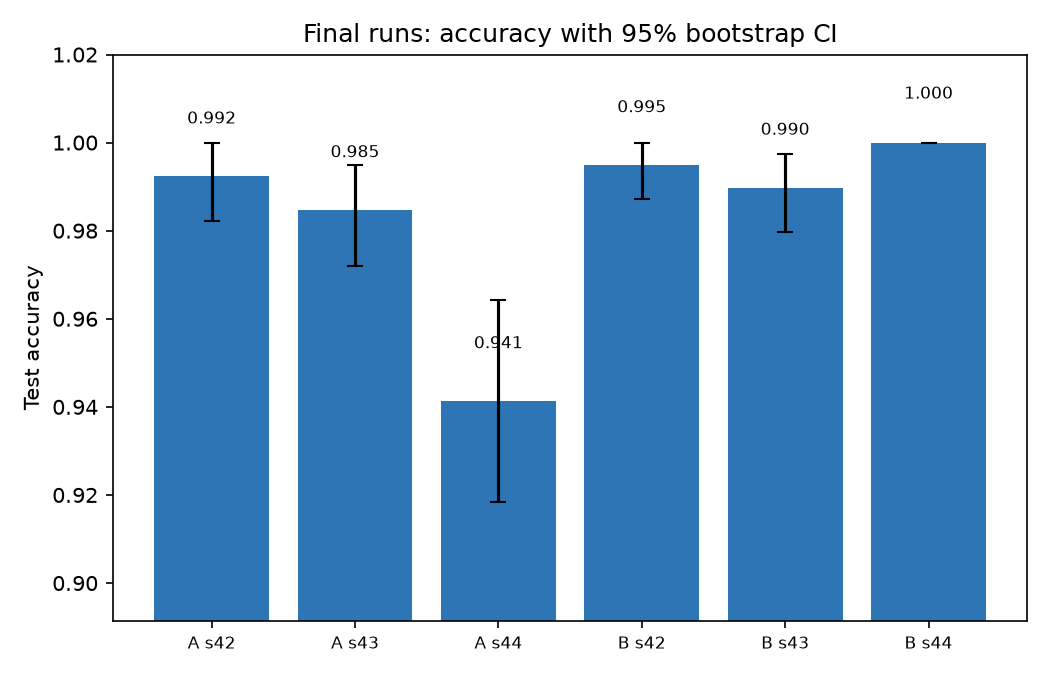
\includegraphics[width=0.78\textwidth]{accuracy_ci.png}
\caption{Test accuracy of the final runs with 95\% percentile bootstrap
confidence intervals (2,000 resamples, seed 42), computed on the identical test
images. Wilson intervals are reported in the text and in
\texttt{outputs/results/stats.json}.}
\label{fig:ci}
\end{figure}

\subsection{Paired tests: is the difference real?}
Table~\ref{tab:stats} reports three seed-matched exact McNemar tests on paired
per-image correctness over the same leak-free test images. Seeds 42 and 43
differ by 1--2 images (2/1 and 6/4 discordant pairs, $p=1.0000$ and $0.7539$),
so those differences are within noise. Seed 44 differs by 23 images
(0.9413 versus 1.0000, 23/0 discordant pairs, $p<0.001$), which is
significant. The honest summary is not ``B always wins'': B is at least as good
on every seed, is significantly better on the seed where A fails, and has much
lower seed variance.

\begin{table}[H]\centering
\caption{Paired comparisons: bootstrap accuracy and exact McNemar tests.
$b$ = A wrong, B correct; $c$ = A correct, B wrong.}
\label{tab:stats}\begin{tabular}{llcccccc l}
\toprule
A & B & n & Acc A & Acc B & $\Delta$ & b/c & McNemar $p$ & Verdict \\
\midrule
A: leakfree & B: leakfree & 392 & 0.9923 & 0.9872 & -0.0051 & 3/5 & 0.7266 & within noise\\
B: frozen & B: noaug & 382 & 0.9948 & 0.9948 & +0.0000 & 1/1 & 1.0000 & within noise \\
\bottomrule
\end{tabular}
\end{table}

\subsection{Released versus leak-free: the leakage finding}
The released split is structurally invalid for a deployment estimate: 454 of
473 source originals span the train/validation/test boundary, and every
validation and test image shares an original with training. The leak-free
re-split removes that overlap (0/473 clusters span splits). The duplicate
audit, not the aggregate accuracy gap, is the proof of leakage.

Aggregate released scores are not uniformly higher. Averaged over the three
seeds, the final Model A scores 0.9747 on released and 0.9728 on leak-free,
while the final EfficientNetB0 scores 0.9930 on released and 0.9949 on
leak-free. The fixed seed-42 A checkpoint shows the opposite direction
(0.9634 released versus 0.9923 leak-free), although its released run used the
15-epoch task budget rather than the 25-epoch leak-free budget. The two test
sets differ in difficulty and class composition, so the
released-minus-leak-free difference is not a clean causal estimate of
inflation. What the audit establishes is that the released split
cannot answer the deployment question, and that a high released score is
partly near-duplicate recognition. We therefore compare models only on the
same split and with the same training budget, and treat the leak-free number
as the valid one.

\subsection{Qualitative analysis: confusion matrices and Grad-CAM}
Figures~\ref{fig:cm} and~\ref{fig:gradcam} show the confusion matrices and
Grad-CAM panels for the final models. The confusion matrices identify which
classes are confused; the Grad-CAM panels show whether the model looks at
lesions and fruit damage or at background. Each heatmap is normalised to
$[0,1]$ and rendered for the predicted class; unused axes are turned off, and
misclassified examples are shown alongside correct ones.

\begin{figure}[H]
\centering
\begin{subfigure}{0.49\textwidth}
  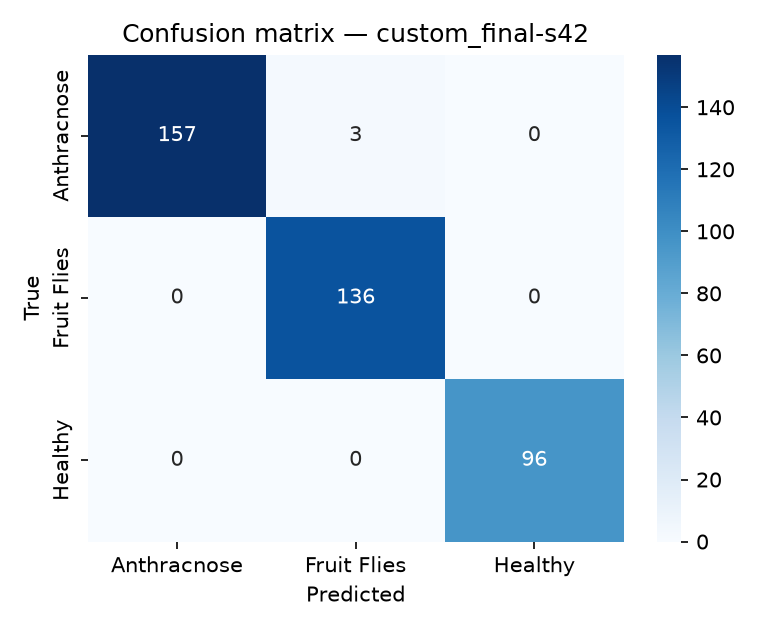
\includegraphics[width=\linewidth]{custom_final-s42_cm.png}
  \caption{Model A, seed 42}
\end{subfigure}
\begin{subfigure}{0.49\textwidth}
  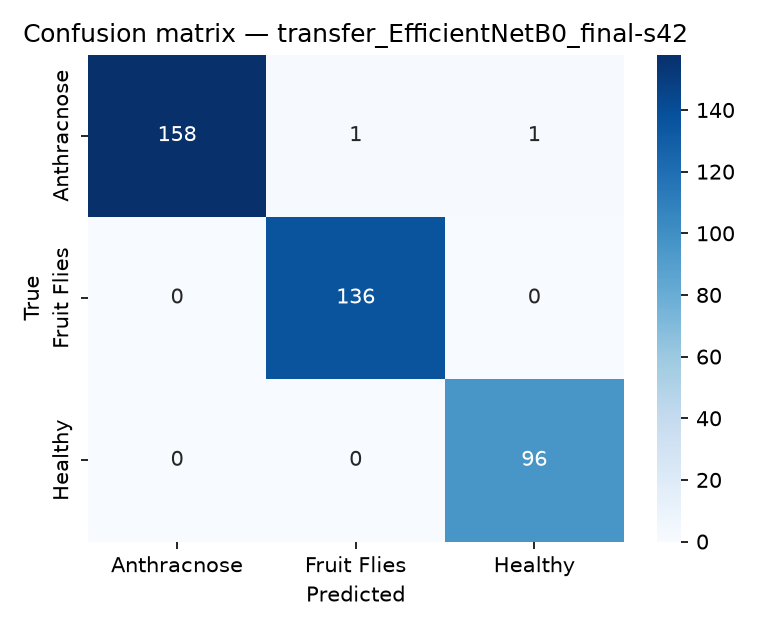
\includegraphics[width=\linewidth]{transfer_EfficientNetB0_final-s42_cm.png}
  \caption{Model B, seed 42}
\end{subfigure}
\caption{Confusion matrices on the leak-free test split (counts).}
\label{fig:cm}
\end{figure}

\begin{figure}[H]
\centering
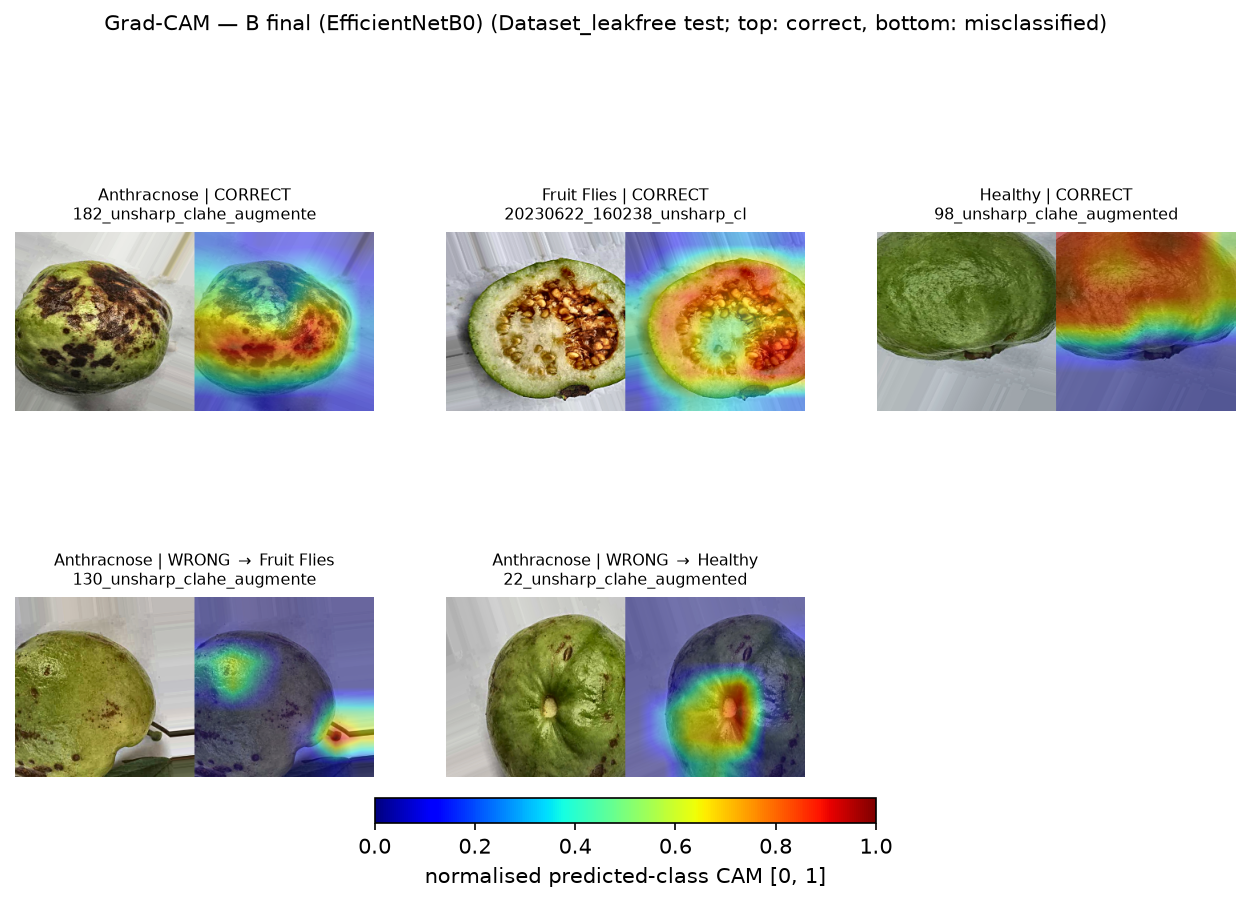
\includegraphics[width=0.96\textwidth]{gradcam_transfer_EfficientNetB0_final-s42_compact.png}
\caption{Grad-CAM for Model B (seed 42, leak-free test). Top row: one correctly
classified example per class. Bottom row: misclassified examples. Colour is the
predicted-class CAM normalised to $[0,1]$ and overlaid on the photograph; the
model label is in the title.}
\label{fig:gradcam}
\end{figure}

\subsection{Bug lessons}
\label{sec:bugs}
Two bugs materially changed the results. First, the augmentation pipeline
rescaled images to $[0,1]$ before applying \texttt{RandomBrightness} and
\texttt{RandomContrast}, whose defaults assume $[0,255]$; training batches
spanned $[0,\sim24]$ while validation stayed in $[0,1]$. The model collapsed to
majority-class guessing (test accuracy 0.445). Setting
\texttt{value\_range=(0,1)} fixed the skew. Second, the custom CNN's
batch-normalisation momentum of 0.99 produced stale moving averages: training
mode reached 0.85 accuracy while inference mode predicted one class for every
input. Momentum 0.9 fixed inference. Both bugs are documented in
\texttt{DECISIONS.md} with the exact symptoms and fixes.

\subsection{Limitations}
The build is CPU-only, so all runs use $224\times224$ inputs rather than the
native $512\times512$, and the optimisation grid is smaller than a GPU budget
would allow. Model A's E5 study covers Adam, SGD, and cosine decay; AdamW and
RMSprop were cut and the cut is recorded. The leak-free re-split is a control,
not a field test: it removes augmentations of the same fruit, but it cannot
simulate a genuinely new orchard, camera, or season. The test set has 392
images, so a one-image difference is 0.26 percentage points; confidence
intervals and McNemar tests are reported for exactly this reason. Finally, the
released split's validation count is 755 on disk versus 775 in the release
notes; we report the discrepancy and do not adjust it.

\section{Conclusion}
We compared a from-scratch CNN with two-phase ImageNet transfer learning on
GFDD24 under a leakage-aware protocol. The released split is fully leaked, so
we built a cluster-grouped leak-free control and tuned only on its validation
split. After fixing an early-stopping bug and a batch-normalisation bug, we ran
a controlled optimisation grid and three seeds per final configuration. The
final comparison is supported by bootstrap confidence intervals and exact
McNemar tests, and the qualitative evidence is shown with Grad-CAM. The
practical lesson is that transfer learning is the stronger default on this
small dataset, although the final A-versus-B difference is only a few test
images and is reported through confidence intervals and McNemar tests. The more
important lesson is methodological: a curated-split accuracy is not a
deployment estimate, and a leak-free control plus paired statistics is the
minimum honest evaluation.

\footnotesize
\raggedright
\bibliographystyle{plainnat}
\bibliography{references}

\end{document}
